\documentclass[12pt]{article}
	\usepackage{amsmath}
	\usepackage{amssymb}
	\usepackage{fancyhdr}
	\usepackage{float}
	\usepackage{graphicx}

	\oddsidemargin0cm
	\topmargin-2cm     %I recommend adding these three lines to increase the 
	\textwidth16.5cm   %amount of usable space on the page (and save trees)
	\textheight23.5cm  

\newcommand{\myname}{Evan Palmer, Titouan Rigoudy}
\newcommand{\myandrew}{esp@andrew.cmu.edu, trigoudy@andrew.cmu.edu}
\newcommand{\myhwnum}{1}
\newcommand{\problemnum}{1}
\newcommand{\thedate}{\today}
\DeclareMathOperator*{\argmax}{arg\,max}
%Page header
	\setlength{\parindent}{0pt}
	\setlength{\parskip}{5pt plus 1pt}
	 
	\pagestyle{fancyplain}
	\lhead{\fancyplain{}{\textbf{HW\myhwnum}}}      % Note the different brackets!
	\rhead{\fancyplain{}{\myname\\ \myandrew}}
	\chead{\fancyplain{}{15-451 }}
\begin{document}
%Title
	\medskip    
	\thispagestyle{plain}
	\begin{center}                 
	{\LARGE Finding The Best Critic For You} \\
	\medskip
	Machine Learning Midterm Report \\
	\smallskip
	\myname \\
	\myandrew \\
	\thedate \\
	\end{center}
	\vspace{0.5cm}


\section{Obtaining the data}

\section{Data descriptions}

\subsection{Rotten tomatoes}

The data we retrieved from Rotten tomatoes included approximately five hundred thousand reviews by about four thousand unique critics about four thousand movies.

Movie stats
loaded data from file
\begin{table}[H]
 \centering
 INSERT TITLE \\
 \begin{tabular}{| l | c | c | c | c |}
 \hline
 &  Min & Max & Mean & Std Dev  \\
 \hline
 Top Critcs & 0 & 56 & 22.41 & 16.06 \\
 Other Critics & 0 & 316 & 92.24 & 68.12 \\
 \hline
 \end{tabular}
 \end{table}

\begin{figure}[H]
    \centering
    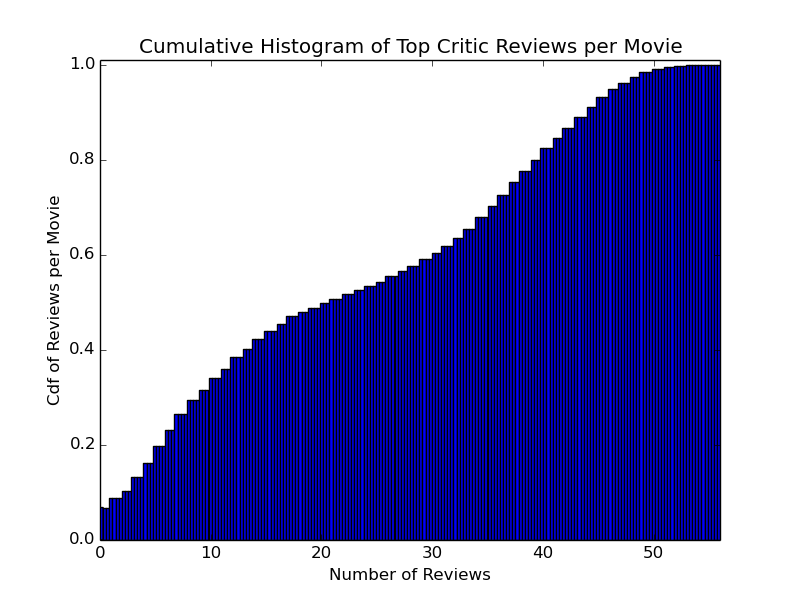
\includegraphics[width=0.48\textwidth]{plots/plot_r_mov_top.png}
    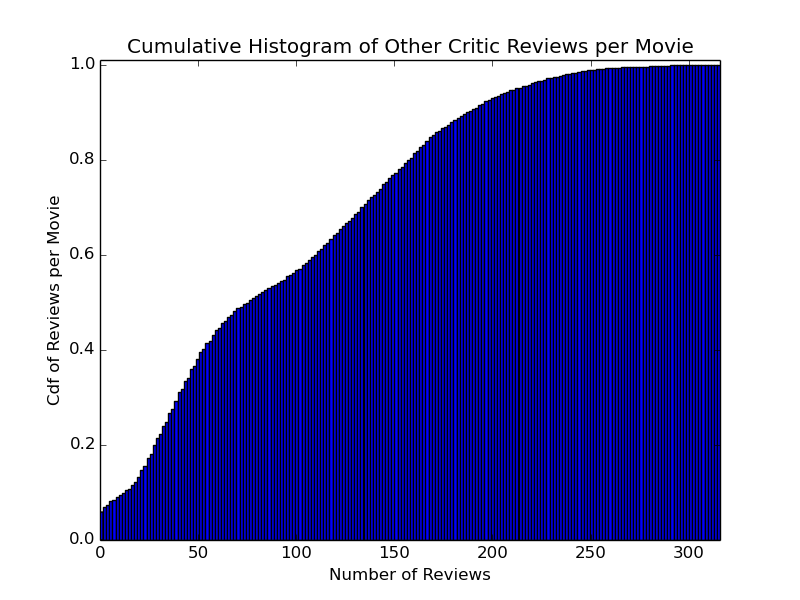
\includegraphics[width=0.48\textwidth]{plots/plot_r_mov_oth.png}
    \caption{INSERT TITLE}
    \label{fig:r_mov}
\end{figure}


Critic stats
loaded data from file
\begin{table}[H]
 \centering
 INSERT TITLE \\
 \begin{tabular}{| l | c | c | c | c |}
 \hline
 &  Min & Max & Mean & Std Dev  \\
 \hline
 Top Critcs & 0 & 2862 & 21.79 & 124.96 \\
 Other Critics & 0 & 2634 & 68.16 & 224.77 \\
 \hline
 \end{tabular}
 \end{table}

\begin{figure}[H]
    \centering
    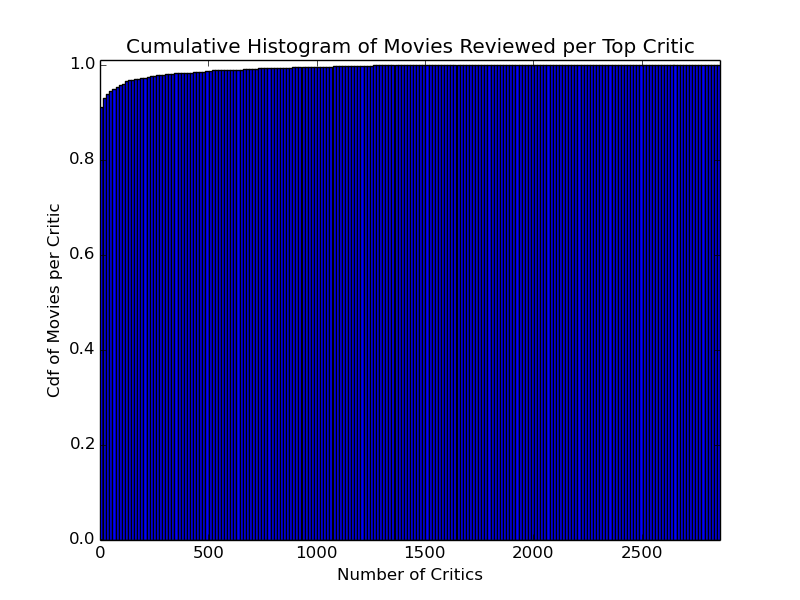
\includegraphics[width=0.48\textwidth]{plots/plot_r_crit_top.png}
    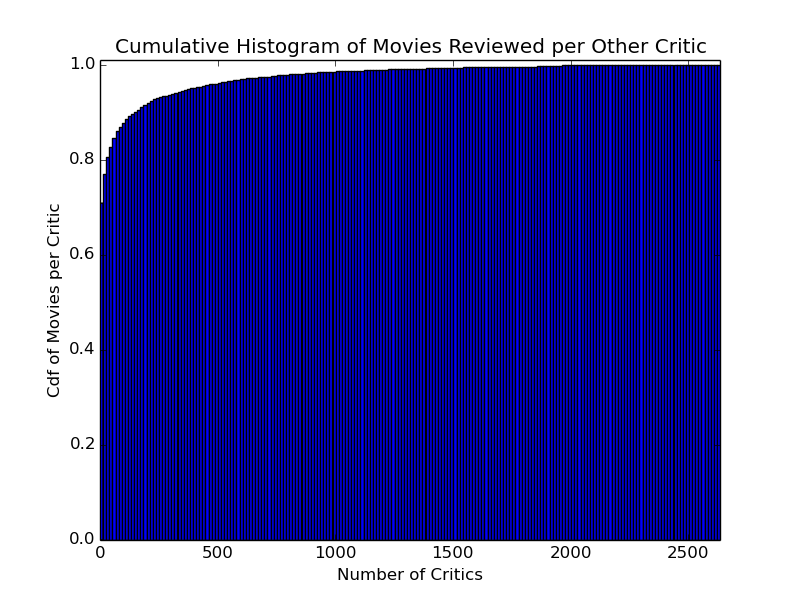
\includegraphics[width=0.48\textwidth]{plots/plot_r_crit_oth.png}
    \caption{INSERT TITLE}
    \label{fig:r_crit}
\end{figure}



Publication stats
loaded data from file
\begin{table}[H]
 \centering
 INSERT TITLE \\
 \begin{tabular}{| l | c | c | c | c |}
 \hline
 &  Min & Max & Mean & Std Dev  \\
 \hline
 Top Publications & 0 & 4135 & 97.22 & 454.15 \\
 Other Publications & 0 & 3224 & 297.78 & 520.28 \\
 \hline
 \end{tabular}
 \end{table}

 \begin{figure}[H]
    \centering
    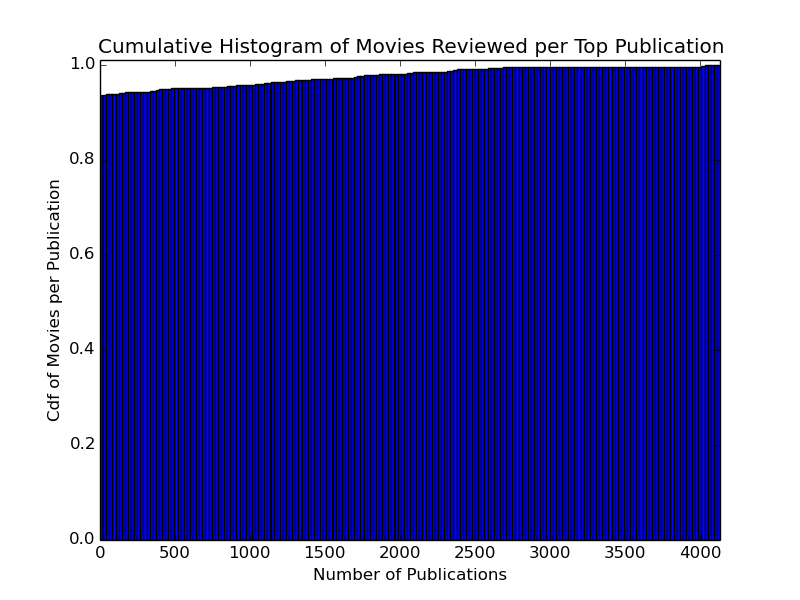
\includegraphics[width=0.48\textwidth]{plots/plot_r_pub_top.png}
    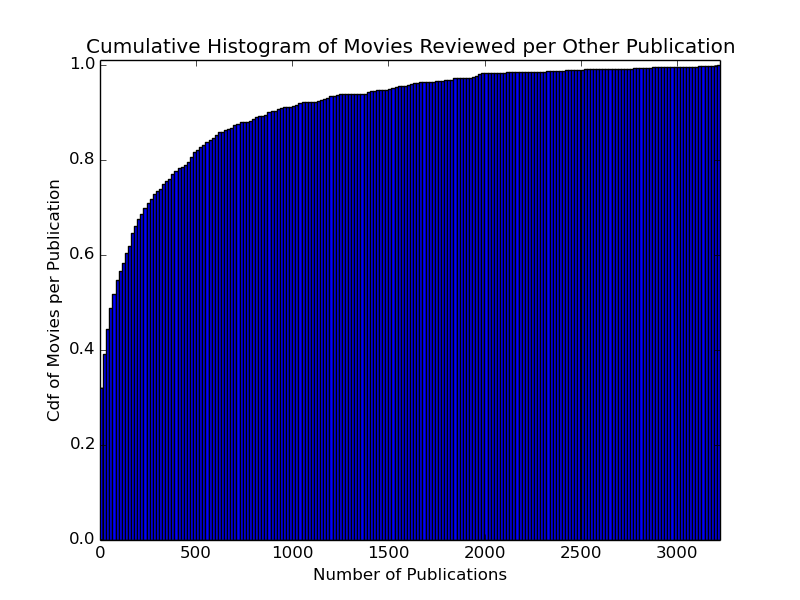
\includegraphics[width=0.48\textwidth]{plots/plot_r_pub_oth.png}
    \caption{INSERT TITLE}
    \label{fig:r_pub}
\end{figure}




\subsection{Metacritic}

Movie stats
\begin{table}[H]
 \centering
 INSERT TITLE \\
 \begin{tabular}{| l | c | c | c | c |}
 \hline
 &  Min & Max & Mean & Std Dev  \\
 \hline
 Critics & 0 & 49 & 25.72 & 10.83 \\
 Users & 0 & 842 & 21.56 & 50.05 \\
 \hline
 \end{tabular}
 \end{table}

 \begin{figure}[H]
    \centering
    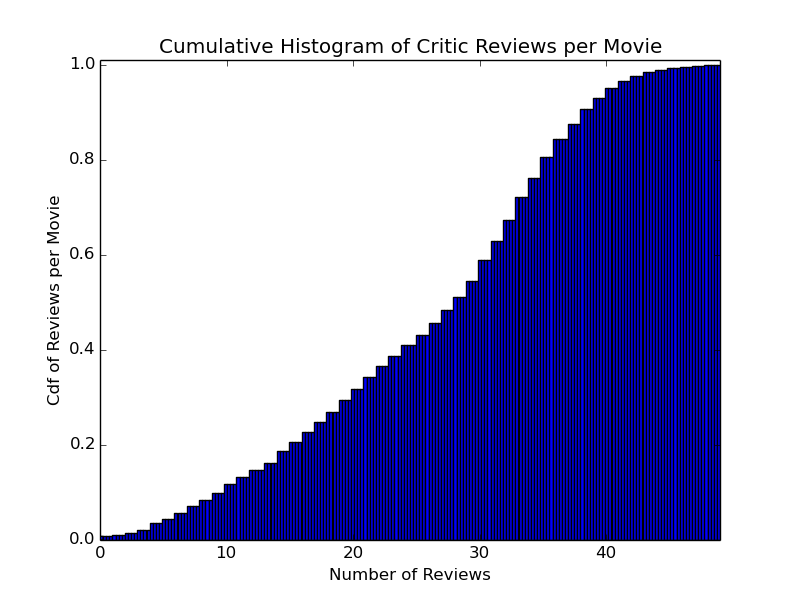
\includegraphics[width=0.48\textwidth]{plots/plot_m_mov_top.png}
    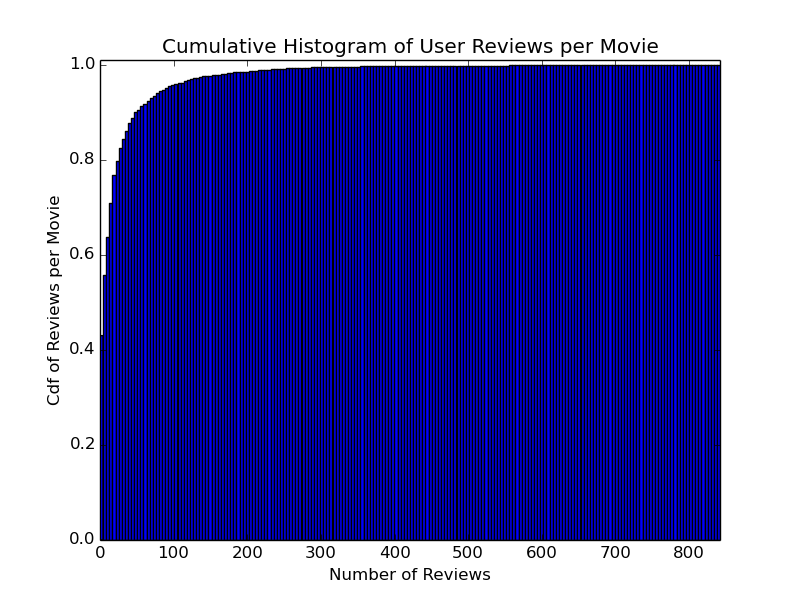
\includegraphics[width=0.48\textwidth]{plots/plot_m_mov_usr.png}
    \caption{INSERT TITLE}
    \label{fig:m_mov}
\end{figure}



User and critic stats
\begin{table}[H]
 \centering
 INSERT TITLE \\
 \begin{tabular}{| l | c | c | c | c |}
 \hline
 &  Min & Max & Mean & Std Dev  \\
 \hline
 Critics & 56 & 3445 & 1203.36 & 912.50 \\
 Users & 1 & 536 & 3.45 & 14.55 \\
 \hline
 \end{tabular}
 \end{table}

 \begin{figure}[H]
    \centering
    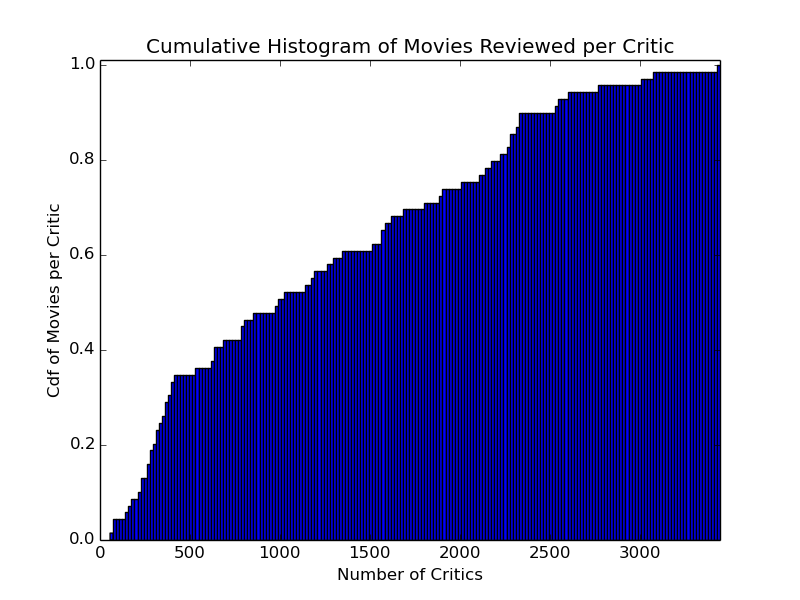
\includegraphics[width=0.48\textwidth]{plots/plot_m_crit_top.png}
    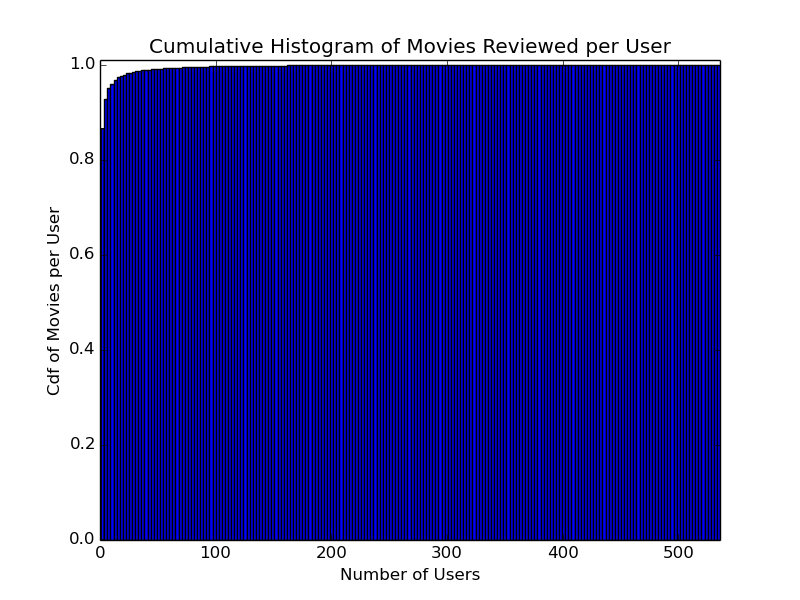
\includegraphics[width=0.48\textwidth]{plots/plot_m_crit_usr.png}
    \caption{INSERT TITLE}
    \label{fig:m_crit}
\end{figure}



\section{Matrix factorization}

\section{Recommender Systems}

\section{Further work}

\end{document}